

\clearpage
\section{Cronograma}
Es la ubicación temporal de las actividades planificadas para la ejecución del proyecto y el logro de los objetivos. Es indispensable que el cronograma sea claro y que los tiempos de ejecución se ajusten a los plazos determinados en la normativa vigente de la Universidad Nacional de Loja. Se recomienda utilizar el diagrama de Gantt, donde se detalla la planificación de las actividades (las que deberán ser planteadas en una secuencia lógica y estar acorde con los objetivos y metodología del proyecto) versus tiempo (Figura \ref{fig:cronograma}).
\begin{figure}[h]
    \centering
    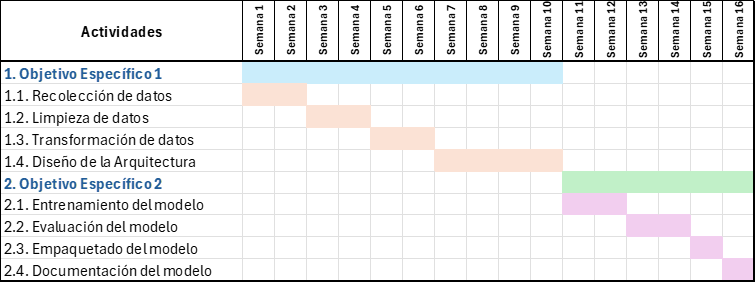
\includegraphics[width=1\linewidth]{imagenes/cronograma.png}
    \caption{Cronograma de actividades}
    \label{fig:cronograma}
\end{figure}
